% В этом документе преамбула

%%% Работа с русским языком
\usepackage{cmap}					% поиск в PDF
\usepackage{mathtext} 				% русские буквы в формулах
\usepackage[T2A]{fontenc}			% кодировка
\usepackage[utf8]{inputenc}			% кодировка исходного текста
\usepackage[english,russian]{babel}	% локализация и переносы
\usepackage{indentfirst}			% чтобы первый абзац в разделе отбивался красной строкой
\frenchspacing						% тонкая настройка пробелов

%%% Приведение начертания букв и знаков к русской типографской традиции
\renewcommand{\epsilon}{\ensuremath{\varepsilon}}
\renewcommand{\phi}{\ensuremath{\varphi}}			% буквы "эпсилон"
\renewcommand{\kappa}{\ensuremath{\varkappa}}		% буквы "каппа"
\renewcommand{\le}{\ensuremath{\leqslant}}			% знак меньше или равно
\renewcommand{\leq}{\ensuremath{\leqslant}}			% знак меньше или равно
\renewcommand{\ge}{\ensuremath{\geqslant}}			% знак больше или равно
\renewcommand{\geq}{\ensuremath{\geqslant}}			% знак больше или равно
\renewcommand{\emptyset}{\varnothing}				% знак пустого множества

%%% Дополнительная работа с математикой
\usepackage{amsmath,amsfonts,amssymb,amsthm,mathtools} % AMS
\usepackage{icomma} % "Умная" запятая: $0,2$ --- число, $0, 2$ --- перечисление

%% Номера формул
\mathtoolsset{showonlyrefs=true} % Показывать номера только у тех формул, на которые есть \eqref{} в тексте.

%% Свои команды

% операции, не определённые (или имеющие иные обохначения) в мат. пакетах
\DeclareMathOperator{\sgn}{\mathop{sgn}}				% ф-ия sgn
\renewcommand{\tg}{\mathop{\mathrm{tg}}\nolimits}		% обозначение тангенса

%% Перенос знаков в формулах (по Львовскому)
\newcommand*{\hm}[1]{#1\nobreak\discretionary{}
{\hbox{$\mathsurround=0pt #1$}}{}}

%%% Работа с картинками
\usepackage{graphicx}  % Для вставки рисунков
\graphicspath{{images/}{images2/}}  % папки с картинками
\setlength\fboxsep{3pt} % Отступ рамки \fbox{} от рисунка
\setlength\fboxrule{1pt} % Толщина линий рамки \fbox{}
\usepackage{wrapfig} % Обтекание рисунков текстом

%%% Работа с таблицами
\usepackage{array,tabularx,tabulary,booktabs} % Дополнительная работа с таблицами
\usepackage{longtable}  % Длинные таблицы
\usepackage{multirow} % Слияние строк в таблице

%%% Теоремы
\theoremstyle{plain} % Это стиль по умолчанию, его можно не переопределять.
\newtheorem{theorem}{Теорема}[section]
\newtheorem{lemma}{Лемма}[section]
\newtheorem{definition}[theorem]{Определение}
\newtheorem{property}{Свойство}
 
\theoremstyle{definition} % "Определение"
\newtheorem{corollary}{Следствие}[theorem]
\newtheorem{exmp}{Пример}[section]
 
\theoremstyle{remark} % "Примечание"
\newtheorem*{nonum}{Решение}
\newtheorem*{evidence}{Доказательство}
\newtheorem*{remark}{Примечание}

%%% Программирование
\usepackage{etoolbox} % логические операторы

%%% Страница
\usepackage{extsizes} % Возможность сделать 14-й шрифт
\usepackage{geometry} % Простой способ задавать поля
	\geometry{top=25mm}
	\geometry{bottom=35mm}
	\geometry{left=35mm}
	\geometry{right=20mm}

%\usepackage{fancyhdr} % Колонтитулы
% 	\pagestyle{fancy}
 	%\renewcommand{\headrulewidth}{0pt}  % Толщина линейки, отчеркивающей верхний колонтитул
% 	\lfoot{Нижний левый}
% 	\rfoot{Нижний правый}
% 	\rhead{Верхний правый}
% 	\chead{Верхний в центре}
% 	\lhead{Верхний левый}
%	\cfoot{Нижний в центре} % По умолчанию здесь номер страницы

\usepackage{setspace} % Интерлиньяж (межстрочные интервалы)
%\onehalfspacing % Интерлиньяж 1.5
%\doublespacing % Интерлиньяж 2
%\singlespacing % Интерлиньяж 1

\usepackage{lastpage} % Узнать, сколько всего страниц в документе.

\usepackage{soulutf8} % Модификаторы начертания

\usepackage{hyperref}
\usepackage[usenames,dvipsnames,svgnames,table,rgb]{xcolor}
\hypersetup{				% Гиперссылки
    unicode=true,           % русские буквы в раздела PDF
    pdftitle={Заголовок},   % Заголовок
    pdfauthor={Автор},      % Автор
    pdfsubject={Тема},      % Тема
    pdfcreator={Создатель}, % Создатель
    pdfproducer={Производитель}, % Производитель
    pdfkeywords={keyword1} {key2} {key3}, % Ключевые слова
    colorlinks=true,       	% false: ссылки в рамках; true: цветные ссылки
    linkcolor=MidnightBlue,          % внутренние ссылки
    citecolor=black,        % на библиографию
    filecolor=magenta,      % на файлы
    urlcolor=blue           % на URL
}

\usepackage{csquotes} % Еще инструменты для ссылок

%\usepackage[style=authoryear,maxcitenames=2,backend=biber,sorting=nty]{biblatex}

\usepackage{multicol} % Несколько колонок

%%% Работа с графикой
\usepackage{tikz}
\usetikzlibrary{calc}
\usepackage{tkz-euclide}
\usetikzlibrary{arrows}
\usepackage{pgfplots}
\usepackage{pgfplotstable}

%%% Настройка подписей к плавающим объектам
\usepackage{floatrow}	% размещение
\usepackage{caption}	% начертание
\captionsetup[figure]{labelfont=bf,textfont=it,font=footnotesize}	% нумерация и надпись курсивом
% для подфигур: заголовок подписи полужирный, текст заголовка обычный
% выравнивание является неровным (т.е. выровненным по левому краю)
% singlelinecheck = off означает, что настройка выравнивания используется, даже если заголовок имеет длину только одну строку.
% если singlelinecheck = on, то заголовок всегда центрируется, когда заголовок состоит только из одной строки.
\captionsetup[subfigure]{labelfont=bf,textfont=normalfont,singlelinecheck=off,justification=raggedright}

%%% Stuff для графиков и рисунков



\DeclareMathOperator{\eq}{\Leftrightarrow}

\title{Приложения современной алгебры}
\date{13.03.2020}
\author{Почаев Никита Алексеевич, гр. 8381 \\ \href{mailto:pochaev.nik@gmail.com}{pochaev.nik@gmail.com} \\ Преподаватель: Дужин Василий Сергеевич}

\begin{document}
	
\renewcommand{\figurename}{Рисунок}

\maketitle

\section{Введение в асимптотическую комбинаторику диаграмм и таблиц Юнга}

\subsection*{Задача 1.}

Вычислить числа разбиений $p(n)$ для $n = 1 \dots 10$ с помощью
\begin{itemize}
	\item Производящей функции;
	\item Рекуррентной формулы.
\end{itemize}

\noindent\textit{Решение:}

\begin{itemize}
	\item Для нахождения $p(n)$ необходимо вычислить коэффициенты при $x^n$ в многочлене, представляющим производящую функцию последовательности (см. теоретические сведения). Очевидно, что при вычислениях не понадобятся множители, в которых $k > n$, а внутри - слагаемые степени $x^j$ при $j > n$.
	
	Таким образом, необходимо раскрыть скобки в произведении вида:
	\[ \prod_{k=1}^n (1 + x^k + x^{2k} + \dots + x^{ik}, ik \le n) \]
	
	Для вычислений использовался математический пакет Wolfram Mathematica. Результат его работы приведён на рис. \ref{fig:img_1}.
	
	\begin{figure}[H]
		\center{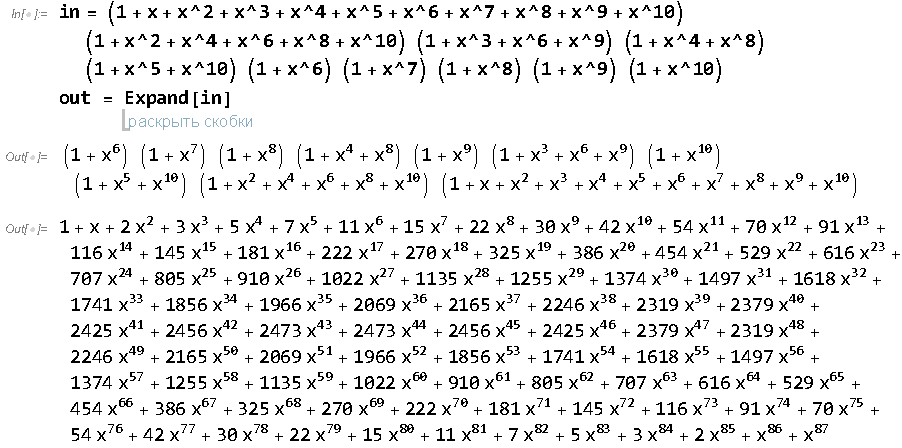
\includegraphics[scale=1]{./media/wolfram_1.pdf}}
		\caption{Раскрытие скобок многочлена}
		\label{fig:img_1}
	\end{figure}

	Обращаясь к последнему выводу, получаем требуемые коэффициенты - число разбиений.
	
	\[ 1 + x + \mathbf{2}x^2 + \mathbf{3}x^3 + \mathbf{5}x^4 + \mathbf{7}x^5 + \mathbf{11}x^6 + \mathbf{15}x^7 + \mathbf{22}x^8 + \mathbf{30}x^9 + \mathbf{42}x^{10} + \dots \]
	
	\item Пользуясь переформулированной пентагольной теоремой Эйлера, вывод которой представлен в разделе "Теоретические сведения"\,, получаем (использование ф-лы расписано для $p(3)$ и $p(5)$):
	\[p(1) = p(0) = 1\]
	
	\[ p(2) = p(1) + p(0) = 1 + 1 = 2 \]
	
	\[ p(3) = (-1)^{1+1} \left(p\left(3-\frac{3-1}{2}\right) + p\left(3-\frac{3+1}{2}\right)\right) + \]
	\[ +(-1)^{1+2}\left(p\left(3-\frac{2(6-2)}{2}\right)+p\left(3-\frac{2(6+1)}{2}\right)\right) = \]
	\[ =p(2) + p(1) - (p(-1) + p(-4)) = p(2) + p(1) = 2 + 1 = 3 \]
	
	\[ p(4) = p(3) + p(2) = 2 + 3 = 5 \]
	
	\[ p(5) = (-1)^{1 + 1} \left(p\left(5-\frac{3-1}{2}\right) + p\left(5-\frac{3+1}{2}\right)\right)+ \]
	\[ + (-1)^{2+1} \left( p\left(5 - \frac{2(6-1)}{2}\right) + p\left(5-\frac{2(6+1)}{2}\right) \right) = \]
	\[ =p(4) + p(3) - (p(0)+p(-2)) = p(4) + p(3) - p(0) = 5 + 3 - 1 = 7 \]
	
	\[ p(6) = p(5) + p(4) - p(1) = 7 + 5 - 1 = 11 \]
	
	\[ p(7) = p(6) + p(5) - p(2) - p(0) = 11 + 7 - 2 - 1 = 15 \]
	
	\[ p(8) = p(7) + p(6) - p(3) - p(1) = 15 + 11 - 3 - 1 = 22 \]
	
	\[ p(9) = p(8) + p(7) - p(4) - p(2) = 22 + 15 - 5 - 2 = 30 \]
	
	\[ p(10) = p(9) + p(8) - p(5) - p(3) = 30 + 22 - 7 - 3 = 42 \]
\end{itemize}

\noindent\textit{Ответ:}

\begin{table}[h]
	\centering
	\begin{tabular}{|c|c|c|c|c|c|c|c|c|c|c|}
		\hline
		$n$    & 1 & 2 & 3 & 4 & 5 & 6  & 7  & 8  & 9  & 10 \\ \hline
		$p(n)$ & 1 & 2 & 3 & 5 & 7 & 11 & 15 & 22 & 30 & 42 \\ \hline
	\end{tabular}
\end{table}

\subsection*{Задача 2.}

Определить соответствия между следующими конструкциями:

\begin{itemize}
	\item Скобочными последовательностями и таблицами Юнга;
	\item Скобочными последовательностями и бинарными деревьями;
	\item Бинарными деревьями и триангуляциями многоугольника.
\end{itemize}

\noindent\textit{Решение:}

\begin{itemize}
	\item Число и тех и других выражается через \underline{числа Каталана}.
	
	Рекуррентная формула для вычисления:
	\[ C_n = \sum_{i=0}^{n-1} C_iC_{n-1-i} \]
	
	Выражение числа Каталана:
	\[ C(n) = \dfrac{(2n)!}{n!(n+1)!} \]
	
	\textit{Правильные скобочные последовательности} – наборы открывающихся и закрывающихся скобок, в которых каждой открывающейся скобке соответствует закрывающаяся. Число возможных последовательностей с фиксированным числом пар скобок выражается числом Каталана. Например, 14 правильных последовательностей из четырех пар скобок:
	\begin{align}
	&(((()))), &((()())), &((())()), &((()))(), &(()(())), &(()()()), &(()())(), \\
	&(())(()), &(())()(), &()((())), &()(()()), &()(())(), &()()(()), &()()()()
	\end{align}
	
	\textit{Таблица (диаграмма) Юнга} - прямоугольник, заполненный последовательными числами так, чтобы они возрастали во всех строках и столбцах. Число таблиц Юнга размером $2 \times n$ выражается числом Каталана.
	\begin{figure}[H]
		\center{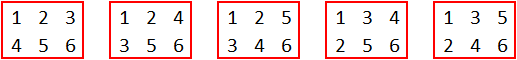
\includegraphics[scale=0.8]{./media/1.2.1.png}}
	\end{figure}

	\noindent\textit{Доказательство:}
	
	Пронумеруем скобки слева направо. Если скобка открывающаяся, то соответствующее ей число пишем в верхнюю строку. Если закрывающаяся, то в – нижнюю. Так как $i$-ая открывающаяся скобка всегда стоит левее $i$-ой закрывающейся, то число соответствующее открывающейся скобке будет меньше числа, соответствующего закрывающей. А значит, верхнее число в таблице окажется меньше нижнего в той же колонке, то есть из правильной скобочной последовательности мы получили таблицу Юнга. Это построение также обратимо, а значит получено взаимно-однозначное соответствие.
	\begin{figure}[H]
		\center{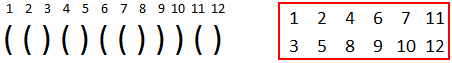
\includegraphics[scale=0.8]{./media/1.2.4.png}}
	\end{figure}

	\item Аналогичная связь с числами Каталана прослеживается с бинарными деревьями. 
	
	\textit{Двоичные деревья} – деревья, из каждого узла которых (кроме листьев) выходит ровно две ветки. Количество бинарных деревьев с заданным числом листьев – число Каталана. На рисунке представлены пять деревьев с 4 листьями в каждом.
	\begin{figure}[H]
		\center{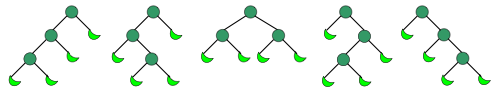
\includegraphics[scale=0.8]{./media/1.2.2.png}}
	\end{figure}

	Количество бинарных деревьев равно:
	\[ C_{n-1} \]

	\noindent\textit{Доказательство:}
	
	Воспользуемся прямым (NLR) обходом дерева и пронумеруем вершины (корень примем за 0) в порядке обхода. Теперь, если при переходе к числу $i$ мы спустились к узлу, являющимся левым для своего родителя, то на $i$-ое место ставим открывающуюся скобку. В противном случае ставим закрывающуюся.
	\begin{figure}[H]
		\center{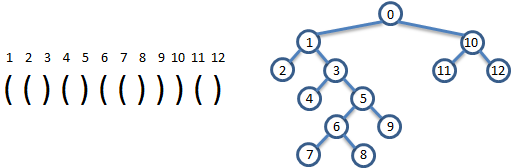
\includegraphics[scale=0.8]{./media/1.2.5.png}}
	\end{figure}
	Дерево – бинарное, поэтому у каждого узла есть сосед. А значит, спустившись к ребенку и поставив открывающуюся скобку, мы рано или поздно доберемся до его соседа и поставим закрывающуюся скобку. Это гарантирует правильность получившейся последовательности. Построение легко обратить и взяв за основу скобочную последовательность получить бинарное дерево.
	Заметим, что если в скобочной последовательности $n$ пар то соответствующее дерево имеет $n+1$ лист.

	\item Количество различных триангуляций выпуклого многоугольника диагоналями равно числу Каталана. $\eq$ Количество разбиений выпуклого $(n + 2)$-угольника на $n$ треугольников непересекающимися диагоналями равно числу Каталана $C_n$.
	
	\textit{Триангуляцией} полигона называется декомпозиция полигона в набор треугольников.
	
	\begin{figure}[H]
		\center{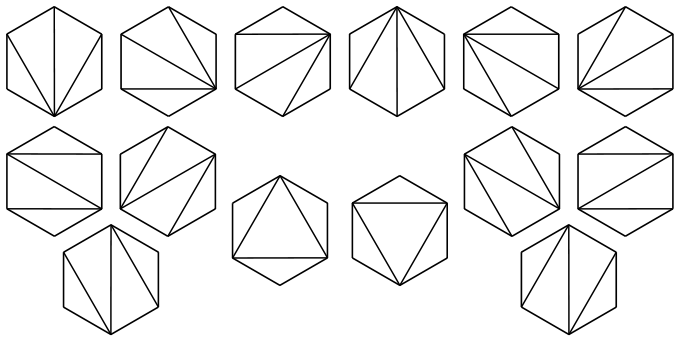
\includegraphics[scale=0.6]{./media/1.2.3.png}}
	\end{figure}

	\noindent\textit{Доказательство:}
	
	Занумеруем в нем все листья слева направо (остальные узлы пометим буквами). Для триангуляции возьмем многоугольник, в котором вершин на одну больше, чем листьев в дереве. Одну из сторон этого многоугольника отметим, как стартовую, а остальные занумеруем (для наглядности – против часовой стрелки).
	Далее выполняем следующую процедуру – если две вершины дерева соседние, то соответствующие стороны многоугольника "стянем"\, диагональю, которую пометим той буквой, которой помечен родитель этой пары узлов в дереве. Далее продолжаем процедуру «стягивания» пока от многоугольника не останется единственный стартовый отрезок.
	\begin{figure}[H]
		\center{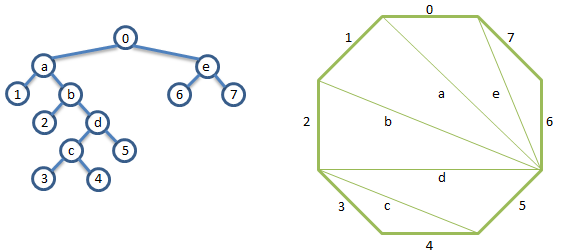
\includegraphics[scale=0.6]{./media/1.2.6.png}}
	\end{figure}
	Как можно заметить три стороны каждого треугольника в получившемся разбиении соответствуют одному родительскому узлу и двум его потомкам. Поэтому, если взять два разных дерева, то получится два разных разбиения.
\end{itemize}

Общее соответствие для 3-его числа Каталана приведено ниже:
\begin{figure}[H]
	\center{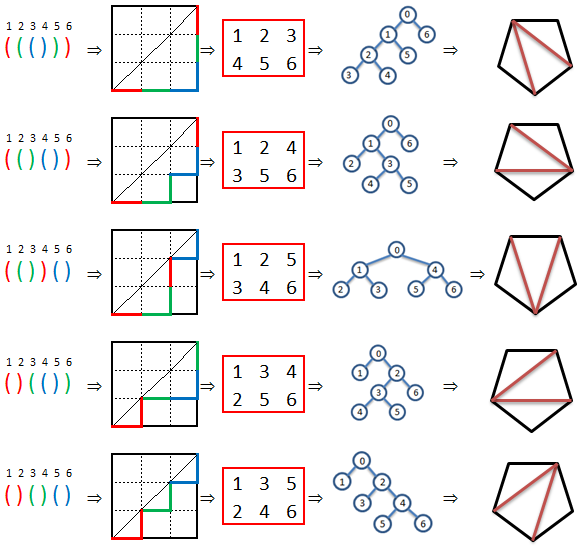
\includegraphics[scale=0.8]{./media/1.2.7.png}}
\end{figure}

\newpage

\section{Соответствие Робинсона-Шенстеда-Кнута}

\subsection*{Задача 1.}

С помощью прямого преобразования RSK сгенерировать таблицы $P, Q$ по следующим перестановкам:
\begin{itemize}
	\item 6, 7, 5, 4, 10, 1, 8, 9, 2, 3
	\item 4, 3, 7, 2, 10, 9, 8, 6, 1, 5
\end{itemize}

\noindent\textit{Решение:}

\begin{figure}[H]
	\center{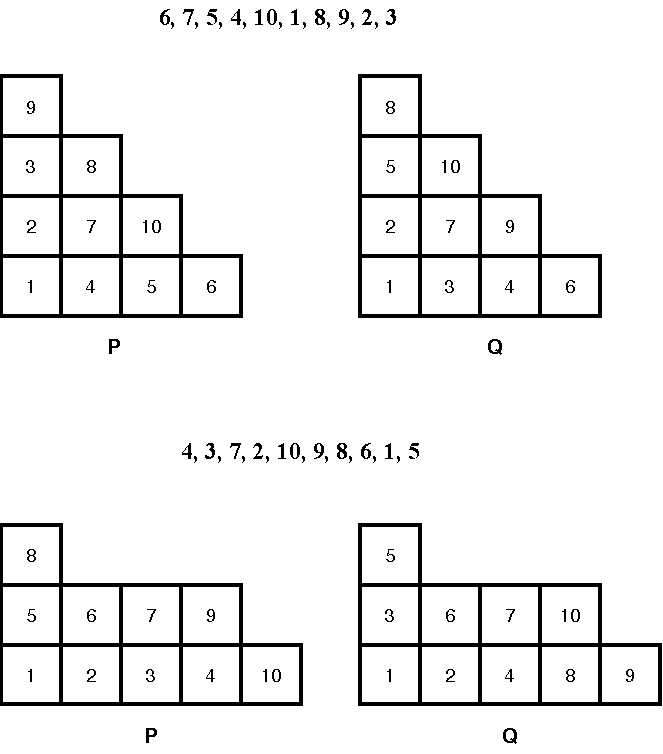
\includegraphics[scale=1]{./media/2.1_1.pdf}}
\end{figure}

\begin{sidewaysfigure}
	\begin{figure}[H]
		\center{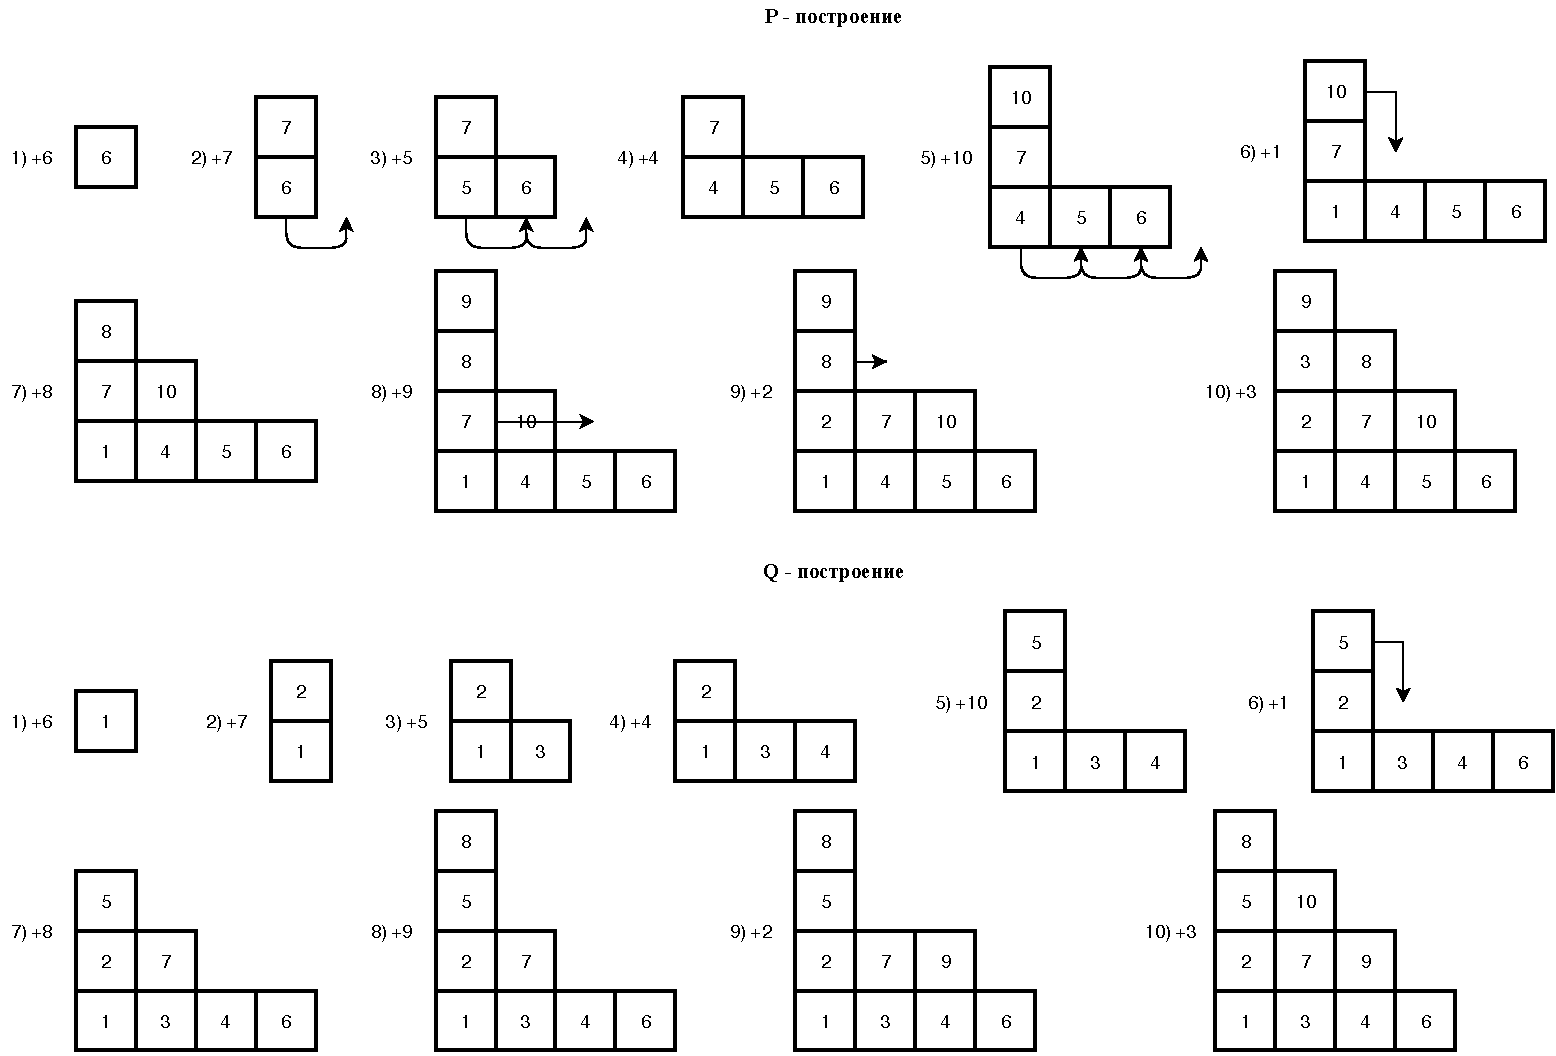
\includegraphics[scale=0.95]{./media/2.1_2.pdf}}
	\end{figure}
\end{sidewaysfigure}

\begin{sidewaysfigure}
	\subsection*{Задача 2.1.}
	\begin{figure}[H]
		\center{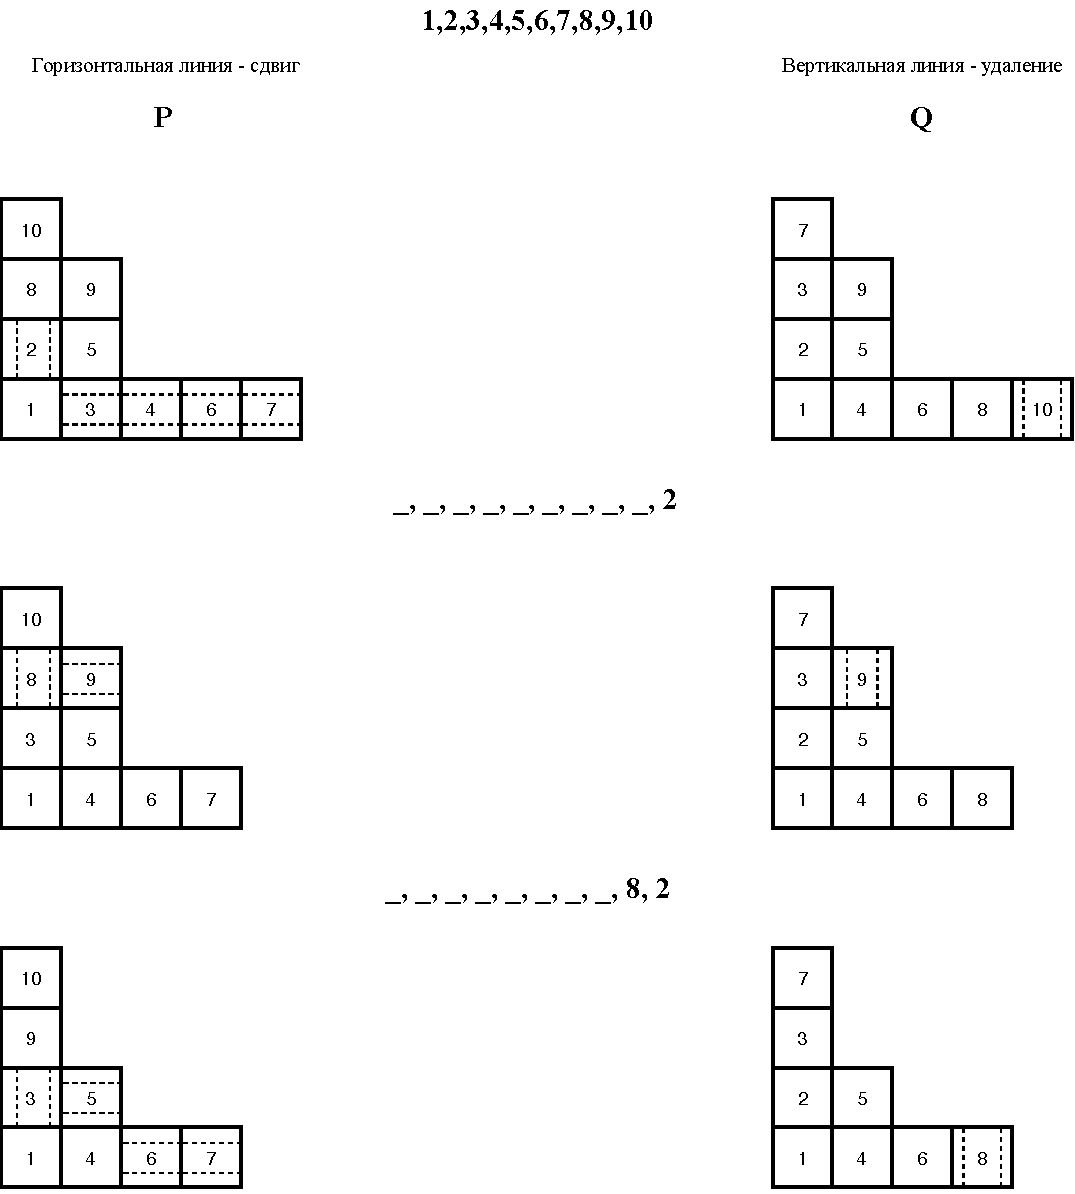
\includegraphics[scale=0.95]{./media/2.2.1_1.pdf}}
	\end{figure}
\end{sidewaysfigure}

\begin{sidewaysfigure}
	\begin{figure}[H]
		\center{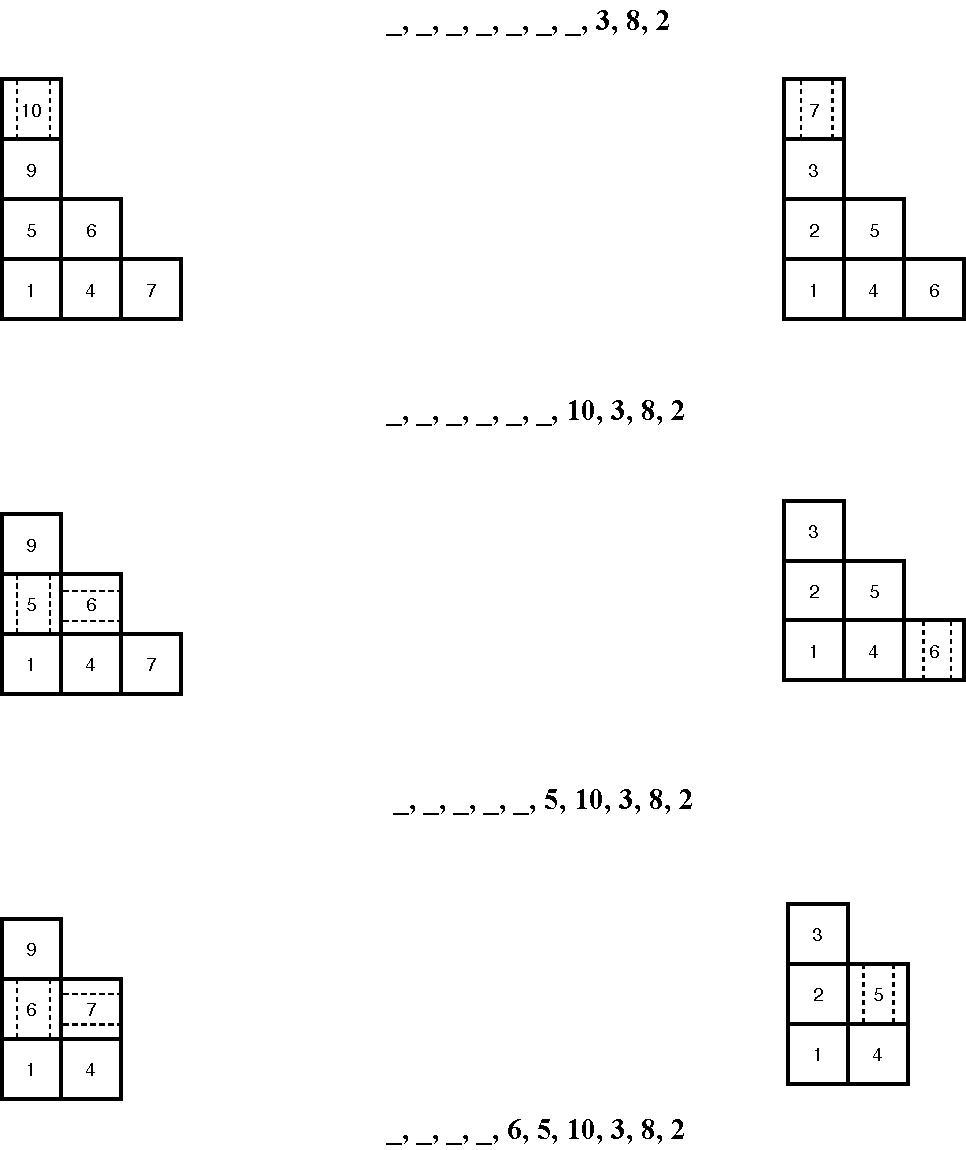
\includegraphics[scale=0.95]{./media/2.2.1_2.pdf}}
	\end{figure}
\end{sidewaysfigure}

\begin{sidewaysfigure}
	\begin{figure}[H]
		\center{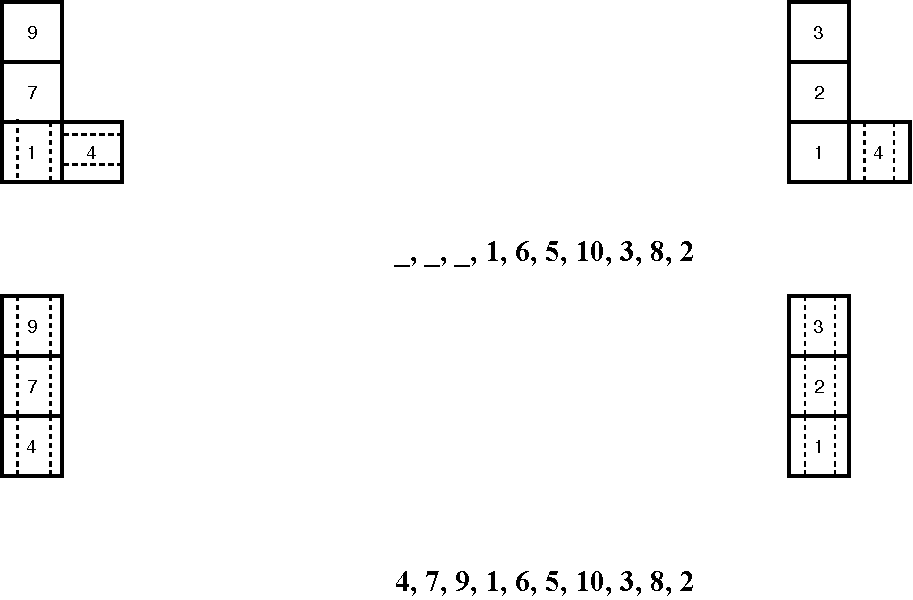
\includegraphics[scale=1]{./media/2.2.1_3.pdf}}
	\end{figure}
\end{sidewaysfigure}

\begin{sidewaysfigure}
	\subsection*{Задача 2.2.}
	\begin{figure}[H]
		\center{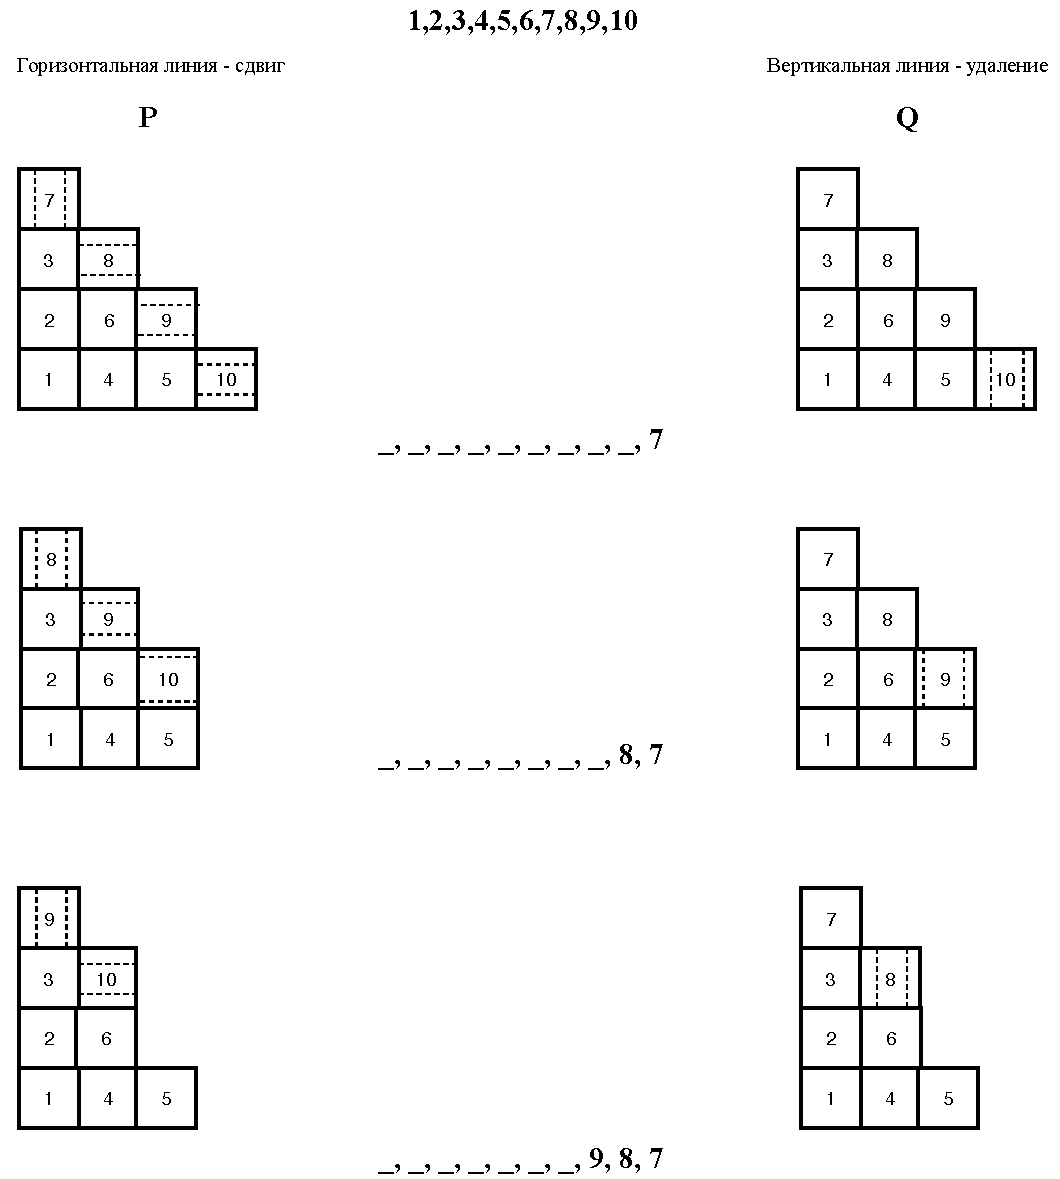
\includegraphics[scale=0.95]{./media/2.2.2_1.pdf}}
	\end{figure}
\end{sidewaysfigure}

\begin{sidewaysfigure}
	\begin{figure}[H]
		\center{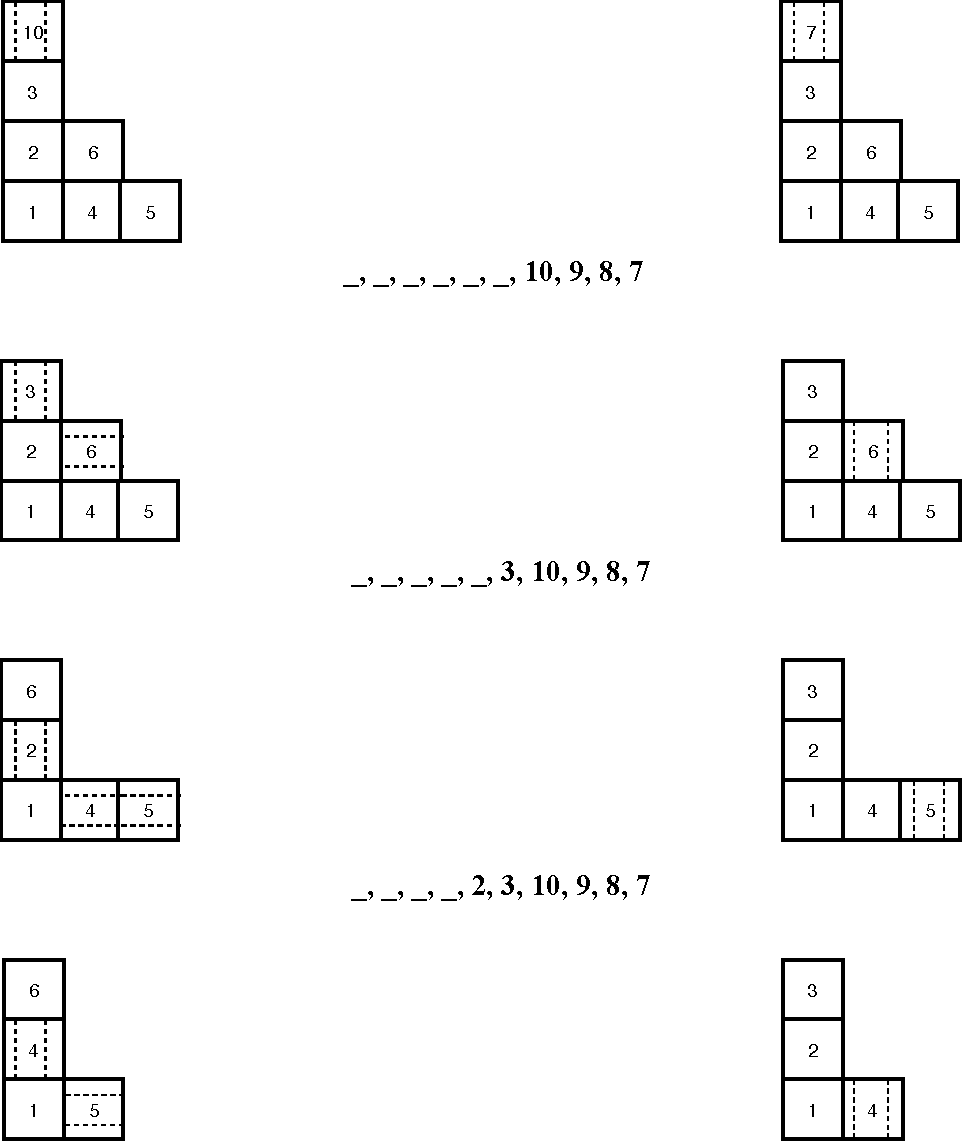
\includegraphics[scale=0.95]{./media/2.2.2_2.pdf}}
	\end{figure}
\end{sidewaysfigure}

\begin{sidewaysfigure}
	\begin{figure}[H]
		\center{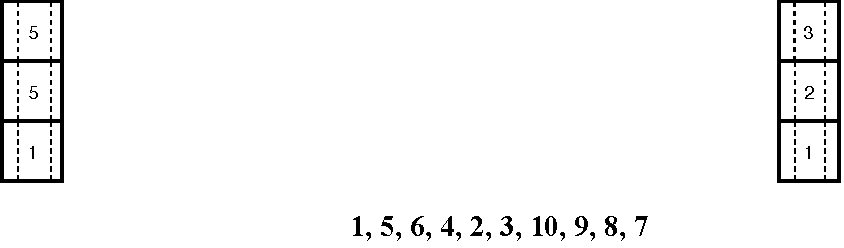
\includegraphics[scale=1]{./media/2.2.2_3.pdf}}
	\end{figure}
\end{sidewaysfigure}

\newpage

\subsection*{Задача 3.}

Выписать все простые подпоследовательности перестановки:
\[ 13, 19, 9, 16, 14, 4, 17, 18, 11, 7, 8, 1, 2, 5, 15, 20, 12, 3, 10, 6 \]
Привести пример возрастающей подпоследовательности максимальной длины.

\noindent\textit{Решение:}

Простые подпоследовательности:
\begin{enumerate}
	\item 13, 9, 4, 1
	\item 19, 16, 14, 11, 7, 2
	\item 17, 8, 5, 3
	\item 18, 15, 12, 10, 6
	\item 20	
\end{enumerate}

\[ N_{\max} = 5 \]

Например: 13, 14, 17, 18, 20.

\section{Преобразование Шютценберже}

\subsection*{Задача 1.}

Нарисовать нервы на приведенных ниже таблицах. Применить к данным таблицам преобразование Шютценберже.
\begin{figure}[H]
	\center{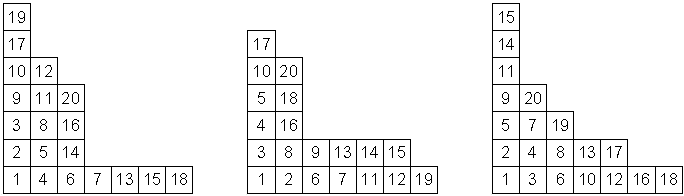
\includegraphics[scale=1]{./media/3.1_task.pdf}}
\end{figure}

\noindent\textit{Решение:}

\begin{figure}[H]
	\center{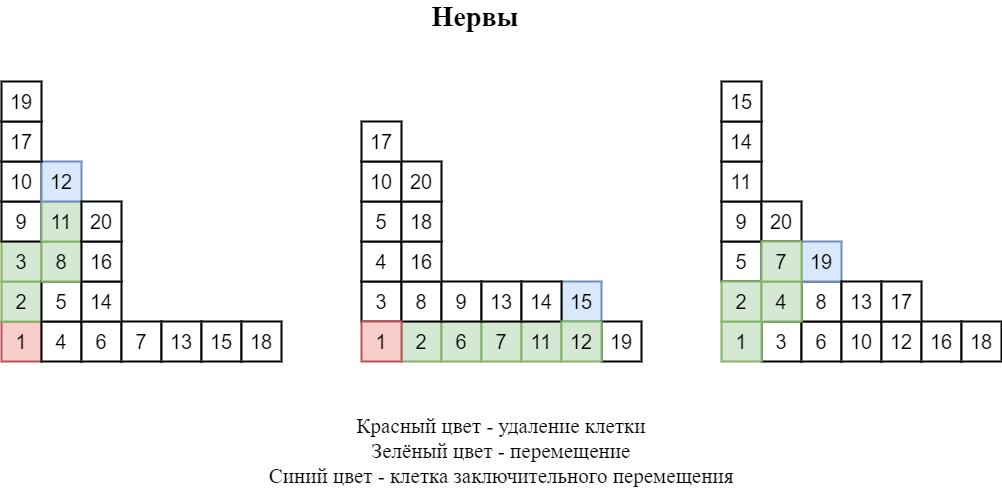
\includegraphics[scale=0.55]{./media/3.1.1.png}}
\end{figure}

\begin{sidewaysfigure}
	\begin{figure}[H]
		\center{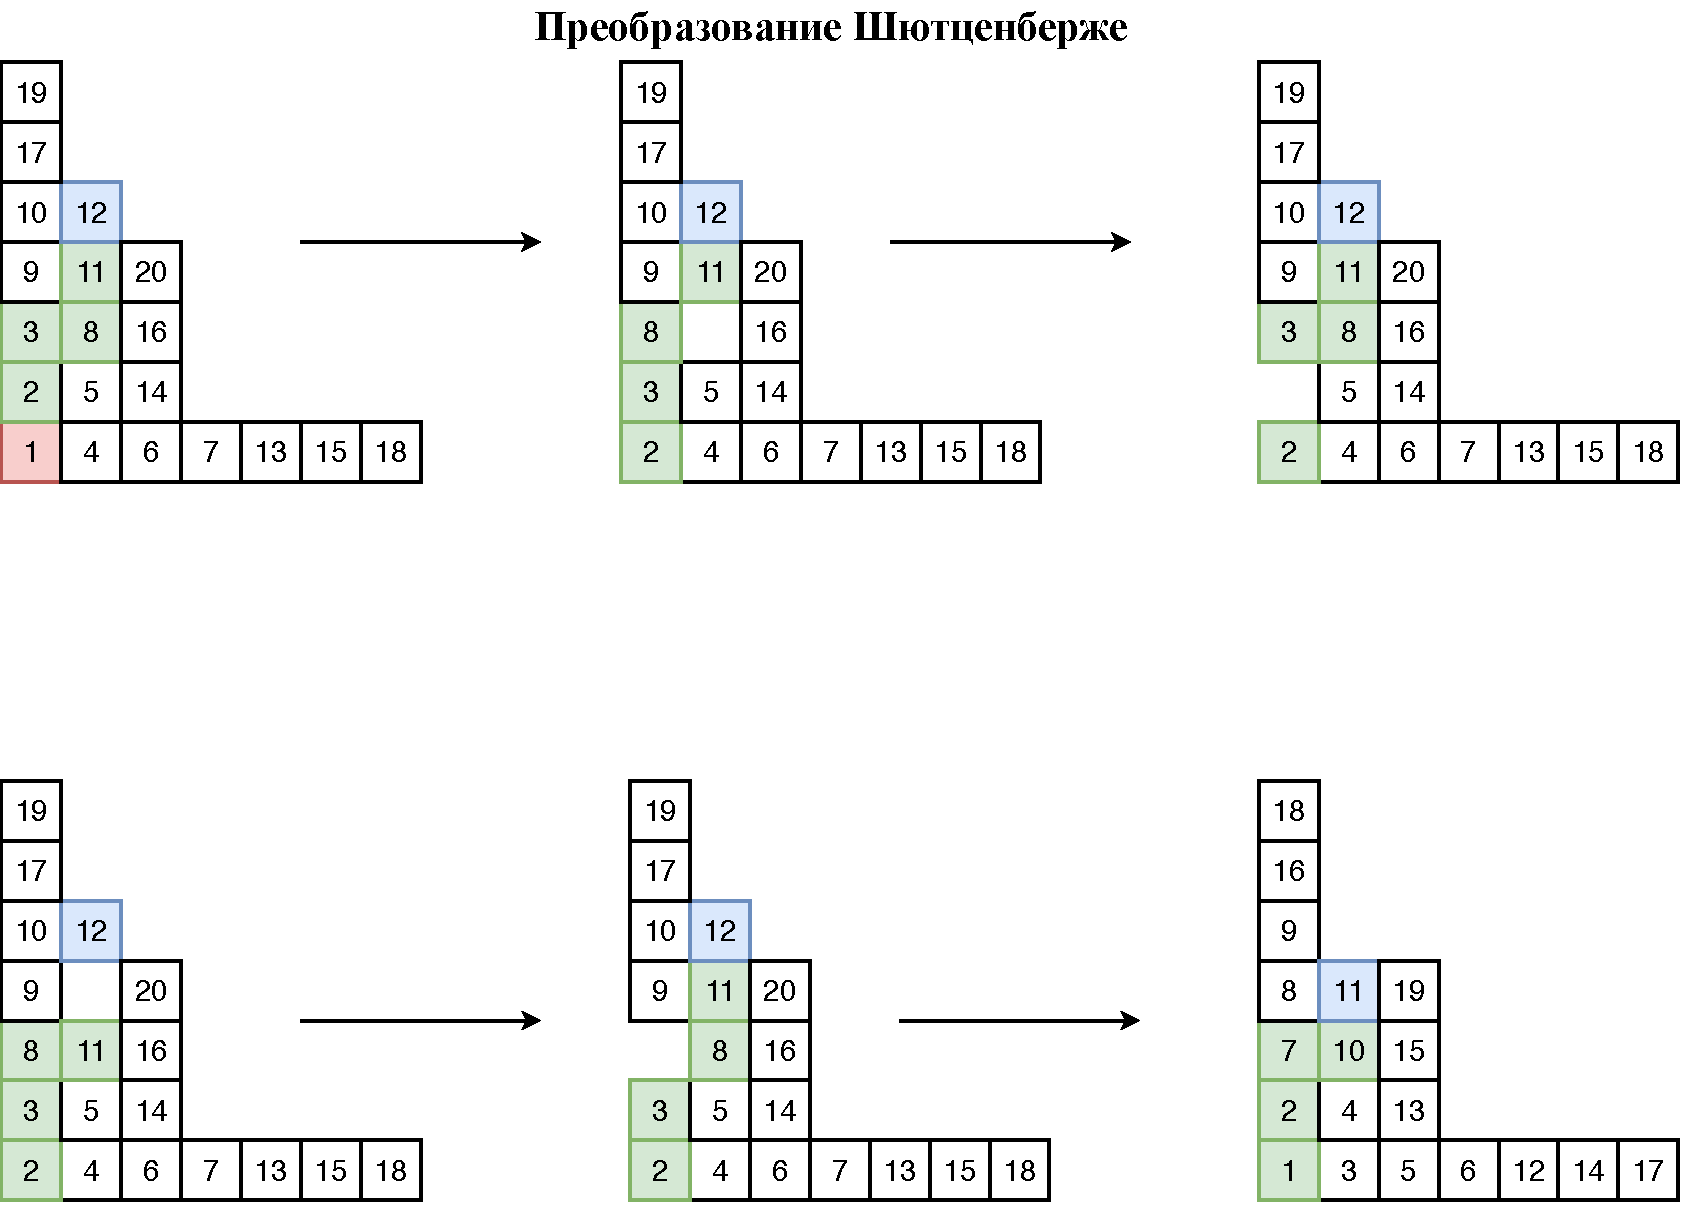
\includegraphics[scale=0.85]{./media/3.1.2.pdf}}
	\end{figure}
\end{sidewaysfigure}

\newpage

\subsection*{Задача 2.}

Дважды применить инволюцию Шютценберже к следующим таблицам Юнга:
\begin{figure}[H]
	\center{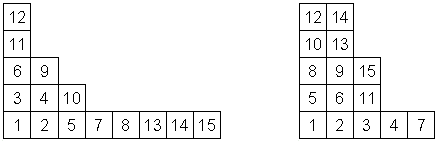
\includegraphics[scale=1]{./media/3.2_task.pdf}}
\end{figure}

\noindent\textit{Решение:}

\begin{sidewaysfigure}
	\begin{figure}[H]
		\center{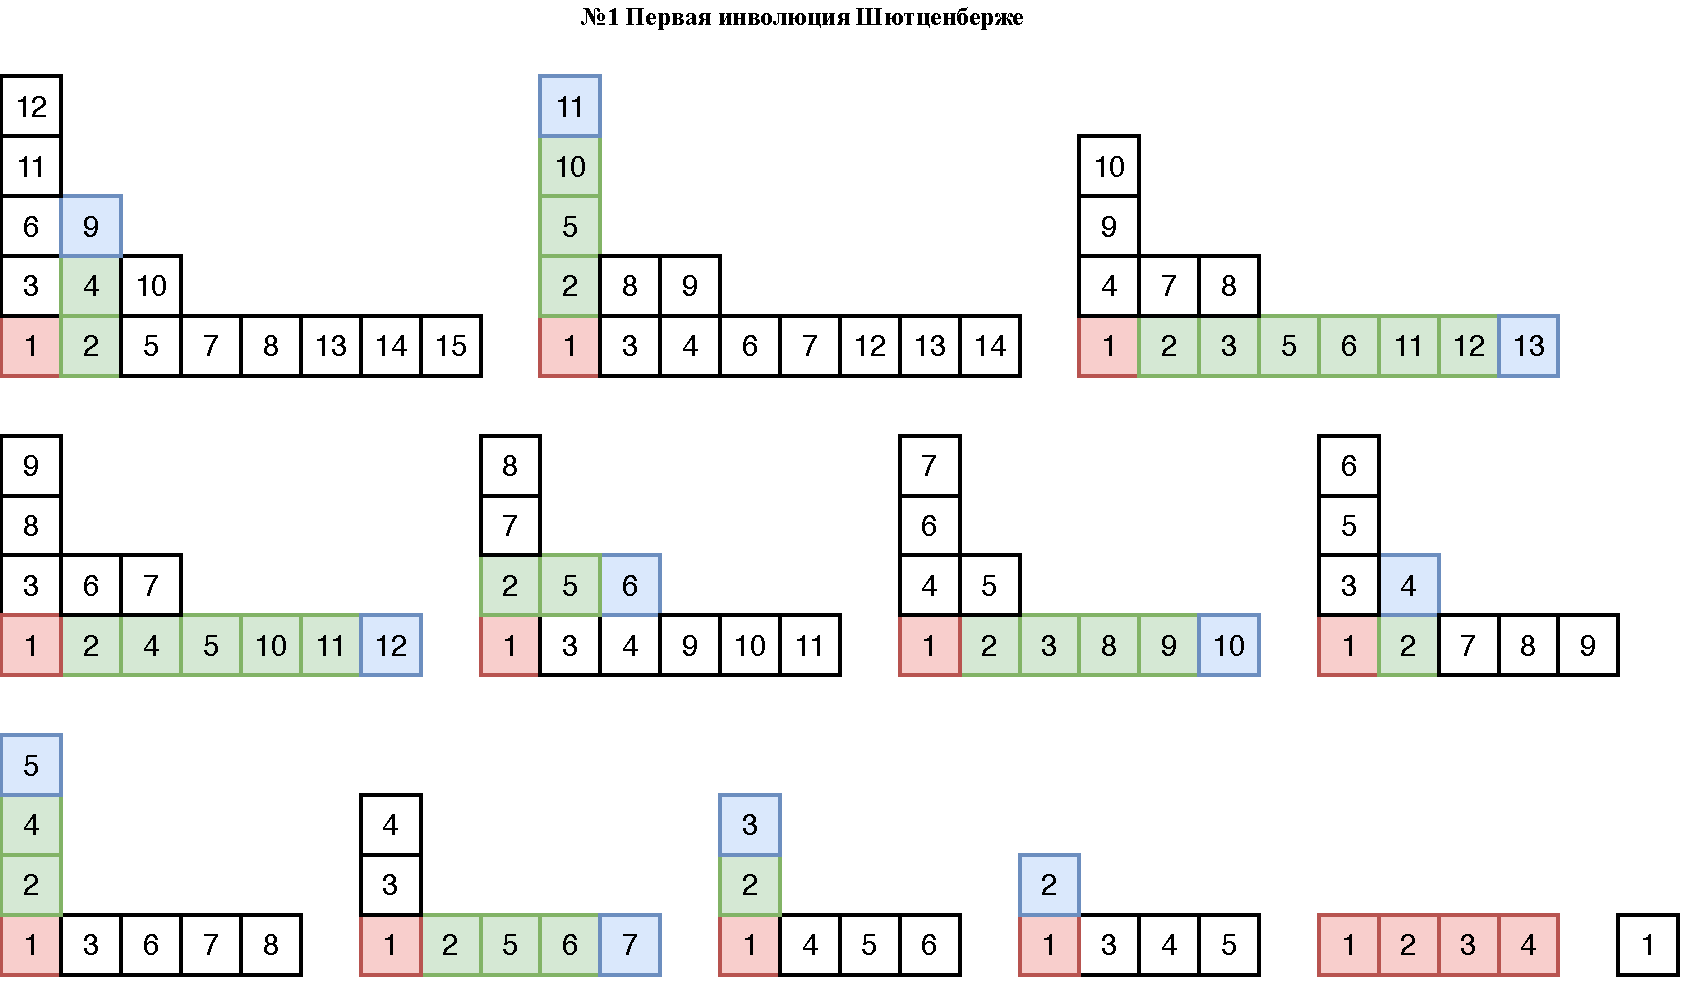
\includegraphics[scale=0.85]{./media/3.2.1.1.pdf}}
	\end{figure}
\end{sidewaysfigure}

\begin{sidewaysfigure}
	\begin{figure}[H]
		\center{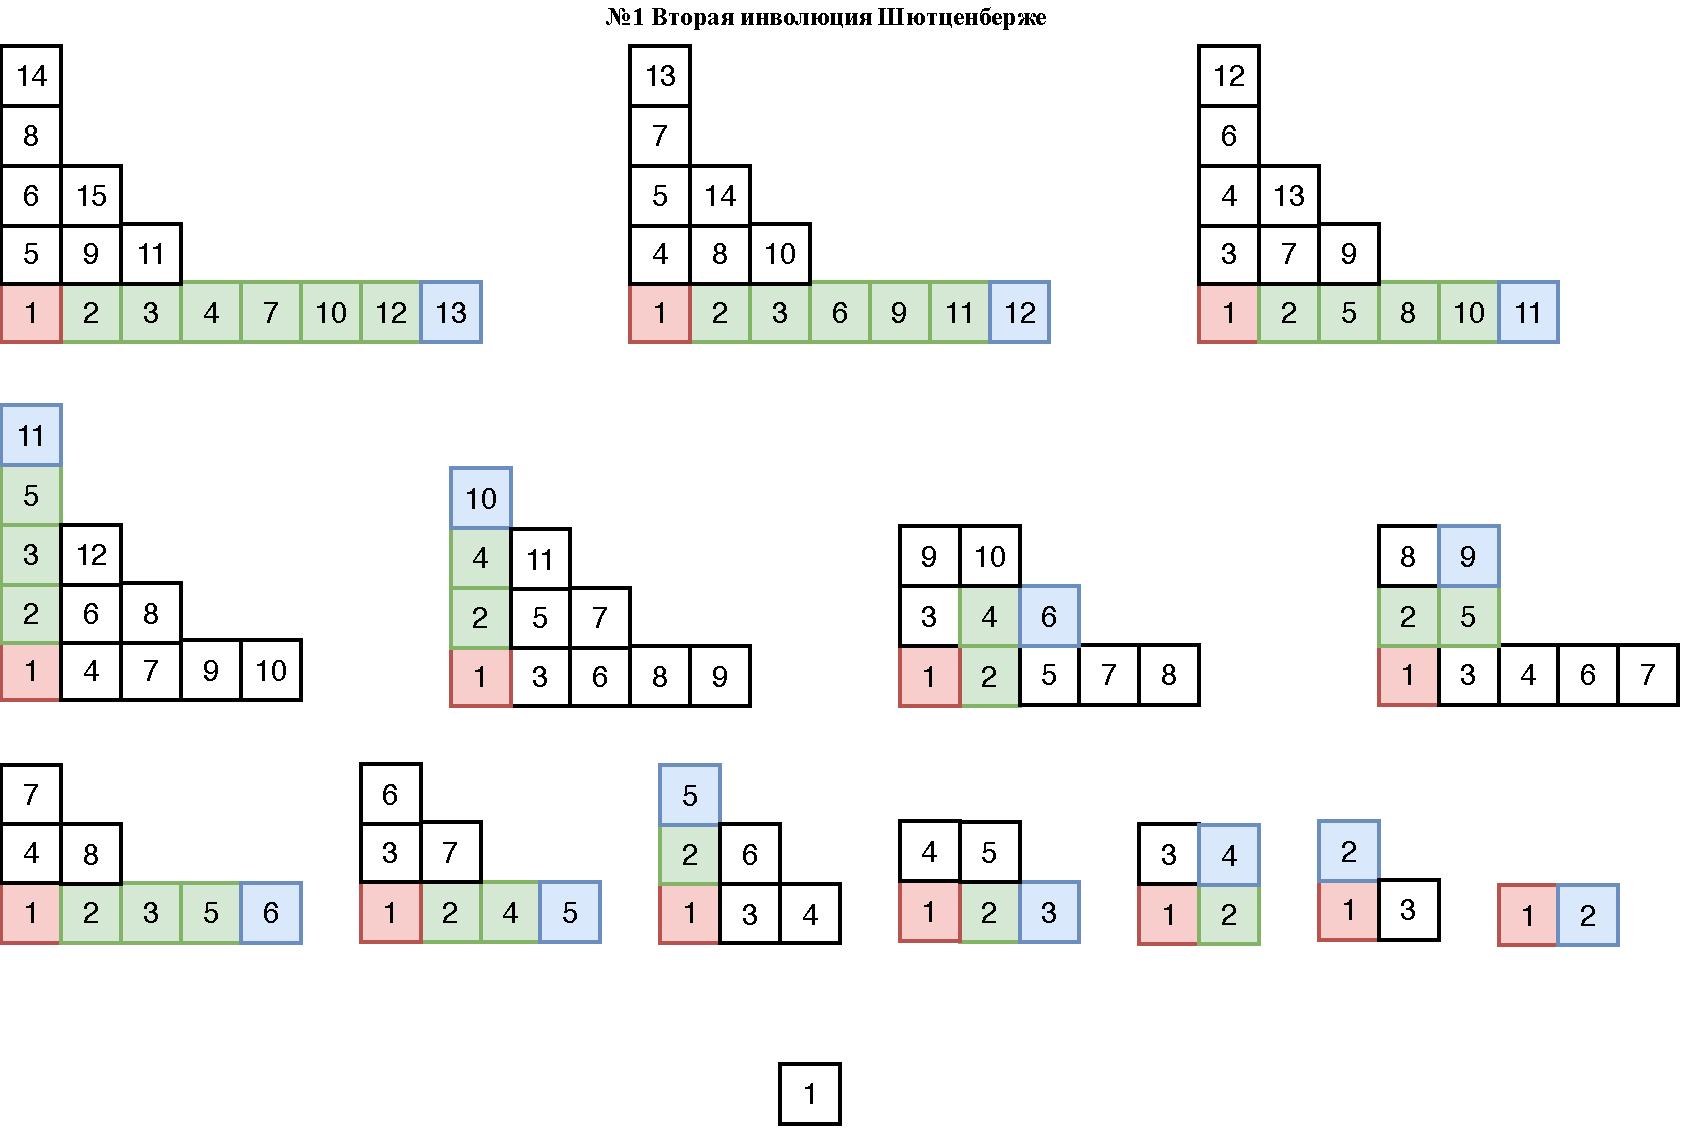
\includegraphics[scale=0.85]{./media/3.2.1.2.pdf}}
	\end{figure}
\end{sidewaysfigure}

\begin{sidewaysfigure}
	\begin{figure}[H]
		\center{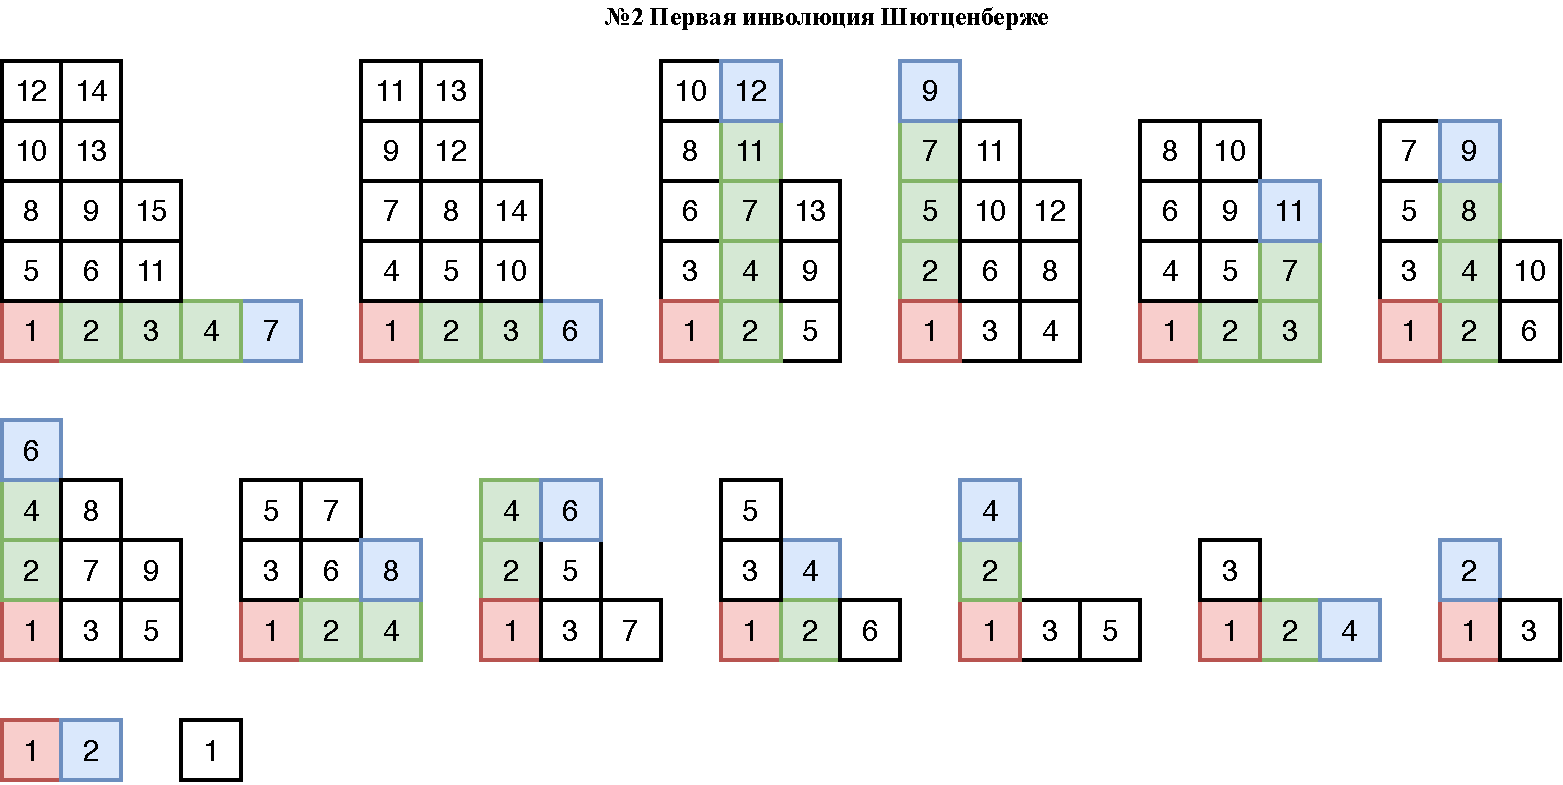
\includegraphics[scale=0.85]{./media/3.2.2.1.pdf}}
	\end{figure}
\end{sidewaysfigure}

\begin{sidewaysfigure}
	\begin{figure}[H]
		\center{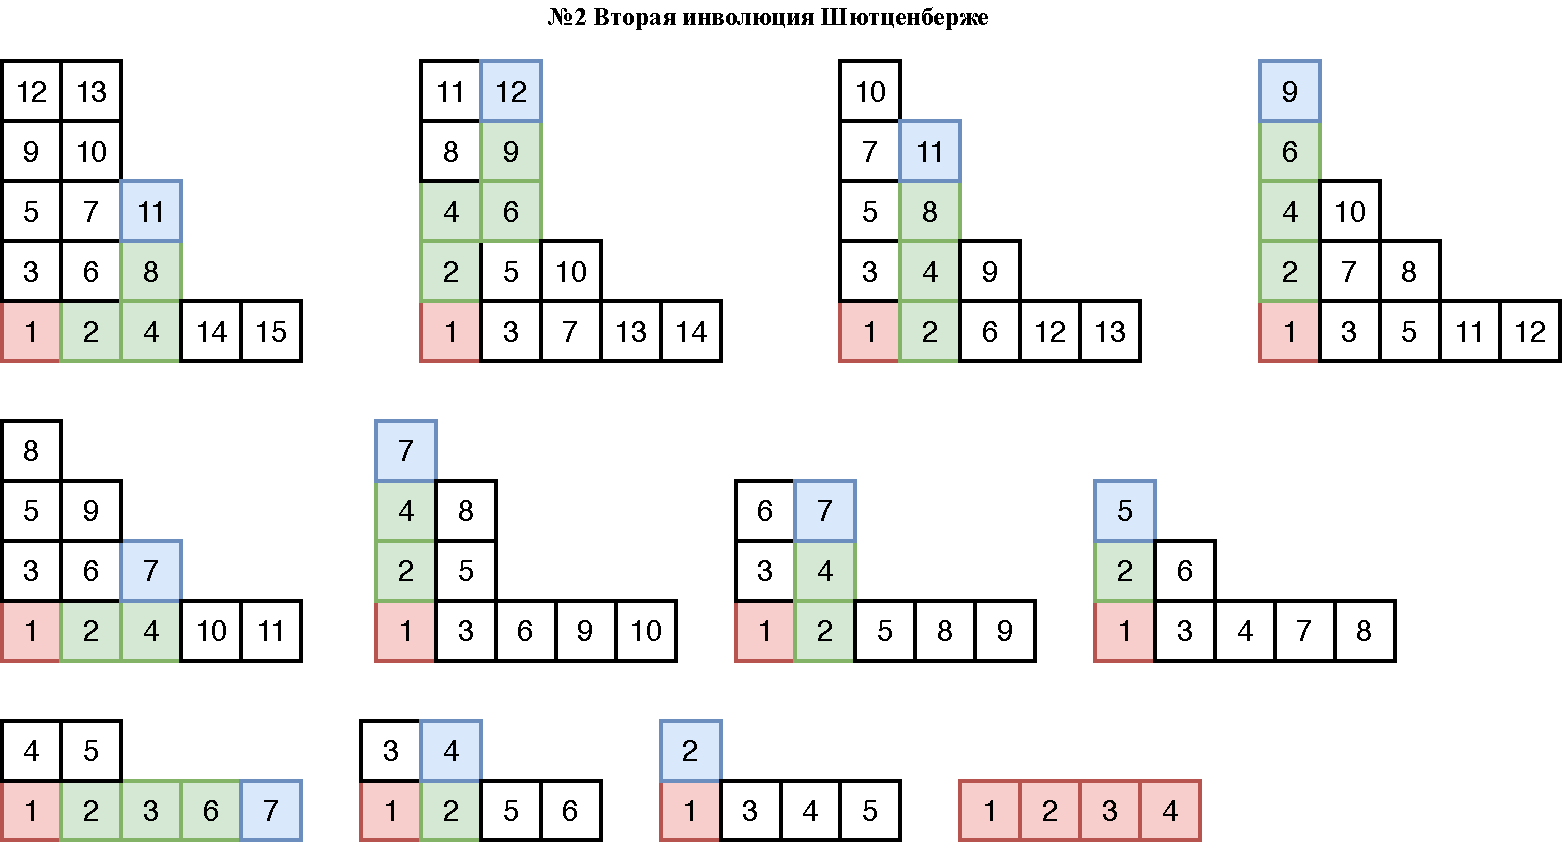
\includegraphics[scale=0.85]{./media/3.2.2.2.pdf}}
	\end{figure}
\end{sidewaysfigure}

\newpage

\subsection*{Задача 3.}

Выписать все возможные трехмерные таблицы Юнга следующей формы:
\begin{figure}[H]
	\center{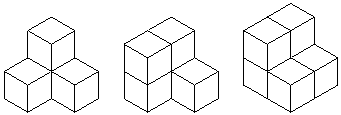
\includegraphics[scale=1]{./media/3.3_task.pdf}}
\end{figure}

С помощью трехмерного преобразования Шютценберже с сохранением формы определить, к каким циклам относятся данные таблицы.

\noindent\textit{Решение:}

Таблицы Юнга для формы размерности 6:
\begin{figure}[H]
	\center{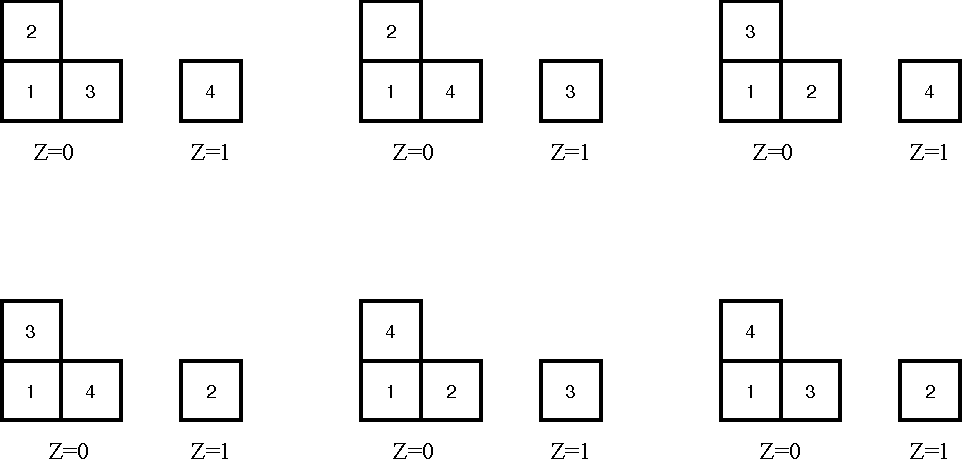
\includegraphics[scale=1]{./media/3.3.1.pdf}}
\end{figure}

При рассмотрении следующей формы ради удобства записи повернём её так, как будто она является модификацией предыдущей: на нижний ярус добавили один блок, чтобы достроить до квадрата.

В итоге таблицы Юнга для формы размерности 8:
\begin{figure}[H]
	\center{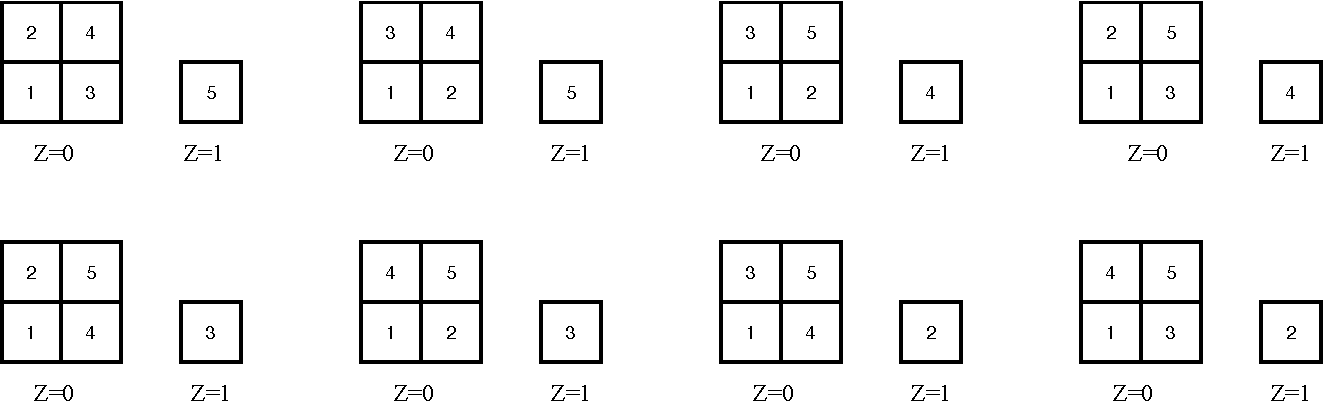
\includegraphics[scale=0.8]{./media/3.3.2.pdf}}
\end{figure}

Таблицы Юнга для формы размерности 16:
\begin{figure}[H]
	\center{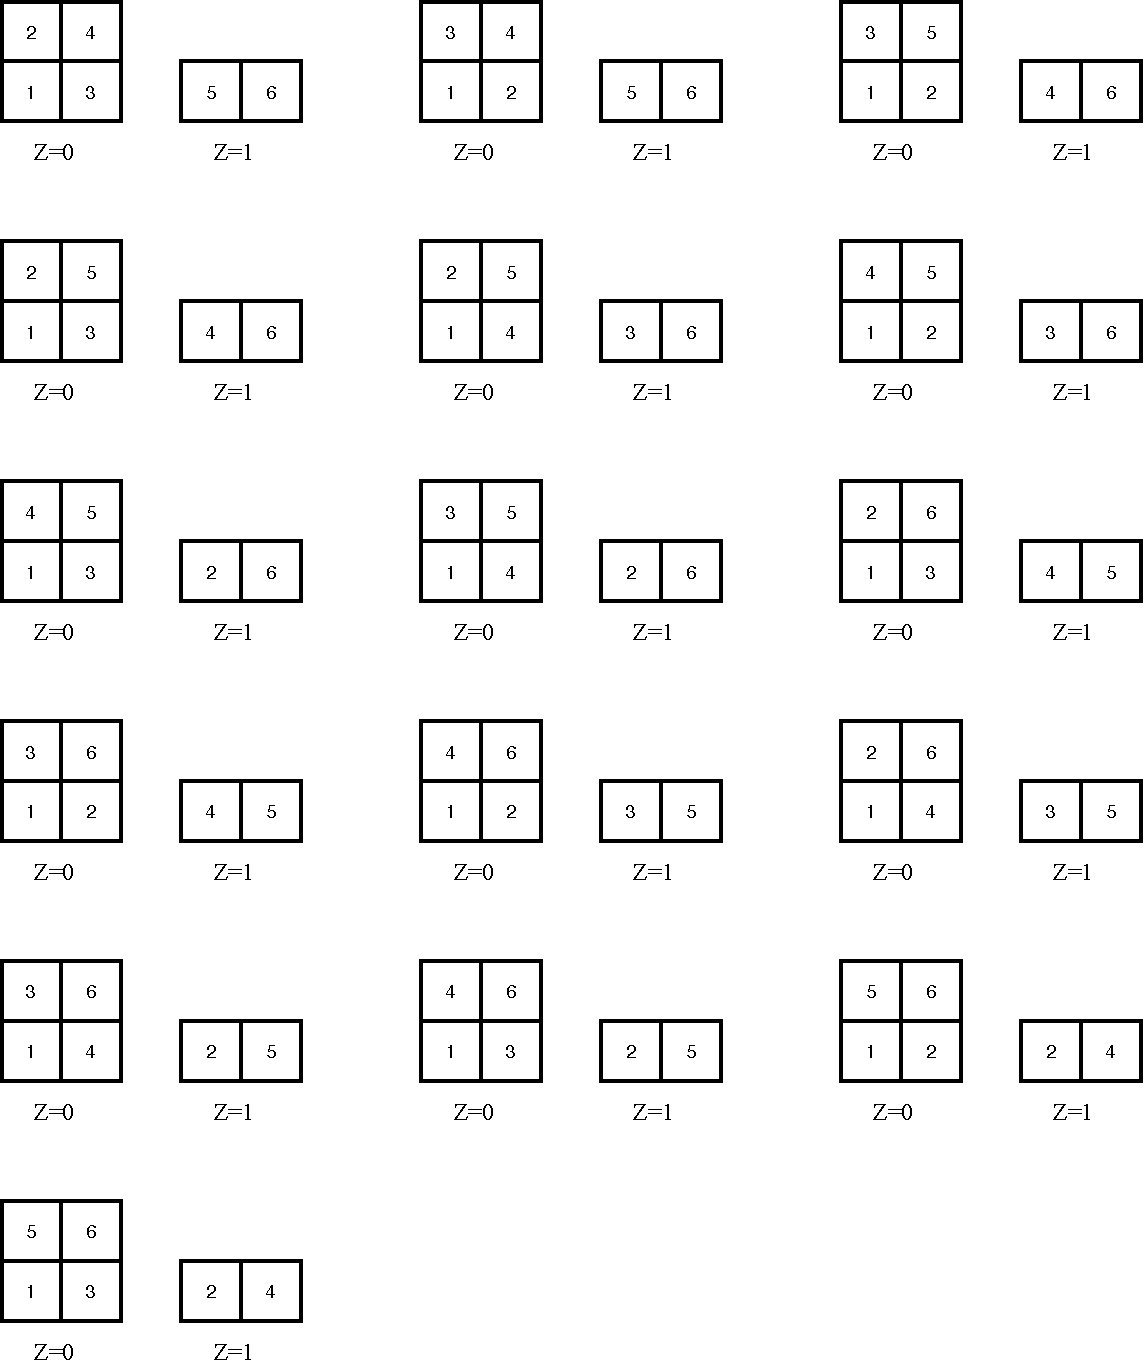
\includegraphics[scale=0.8]{./media/3.3.3.pdf}}
\end{figure}

С помощью трехмерного преобразования Шютценберже с сохранением формы определиv, к каким циклам относятся данные таблицы.

Циклы для 1-ой формы:
\begin{figure}[H]
	\center{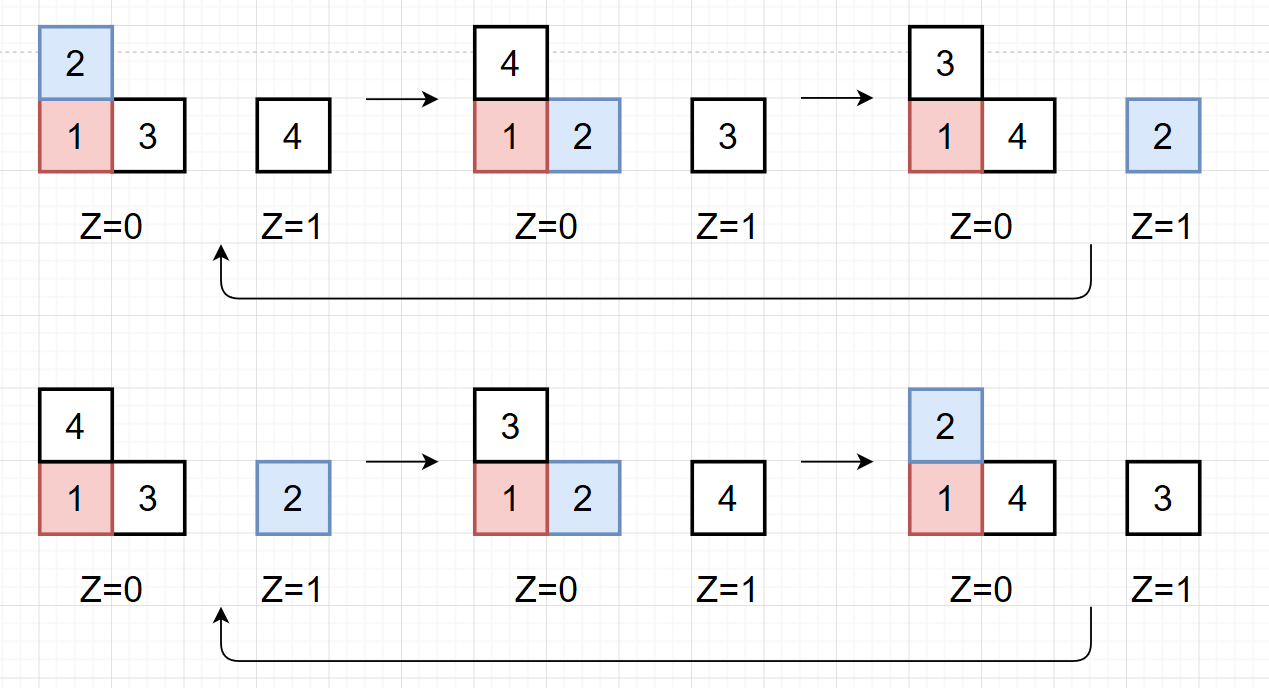
\includegraphics[scale=0.5]{./media/3.3.3_1.png}}
\end{figure}

Цикл для 2-ой формы:
\begin{figure}[H]
	\center{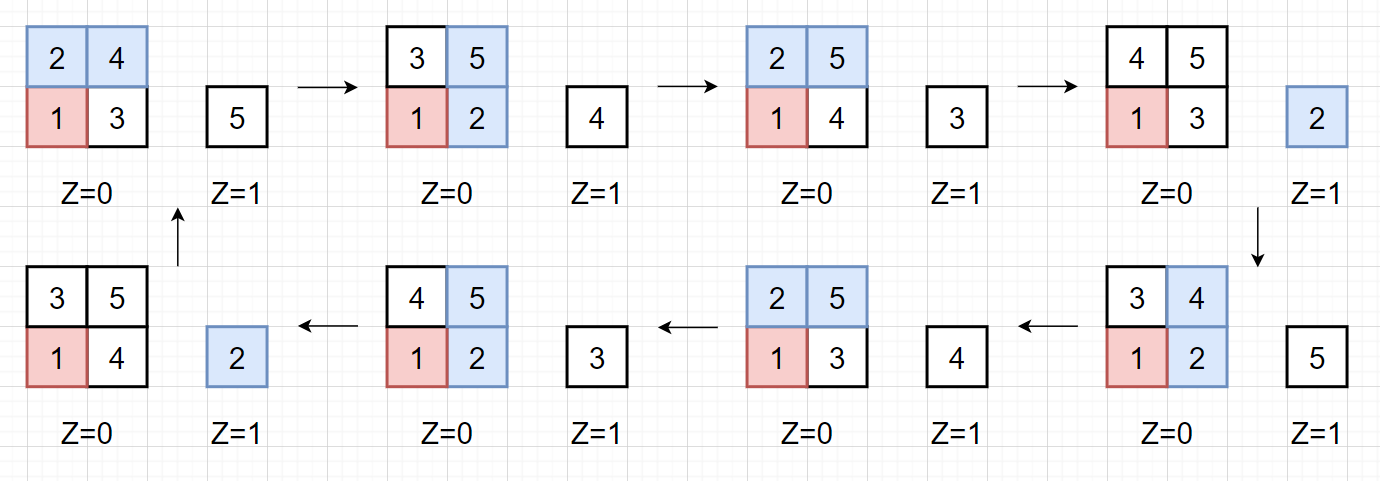
\includegraphics[scale=0.5]{./media/3.3.3_2.png}}
\end{figure}

Цикл для 3-ей формы:
\begin{figure}[H]
	\center{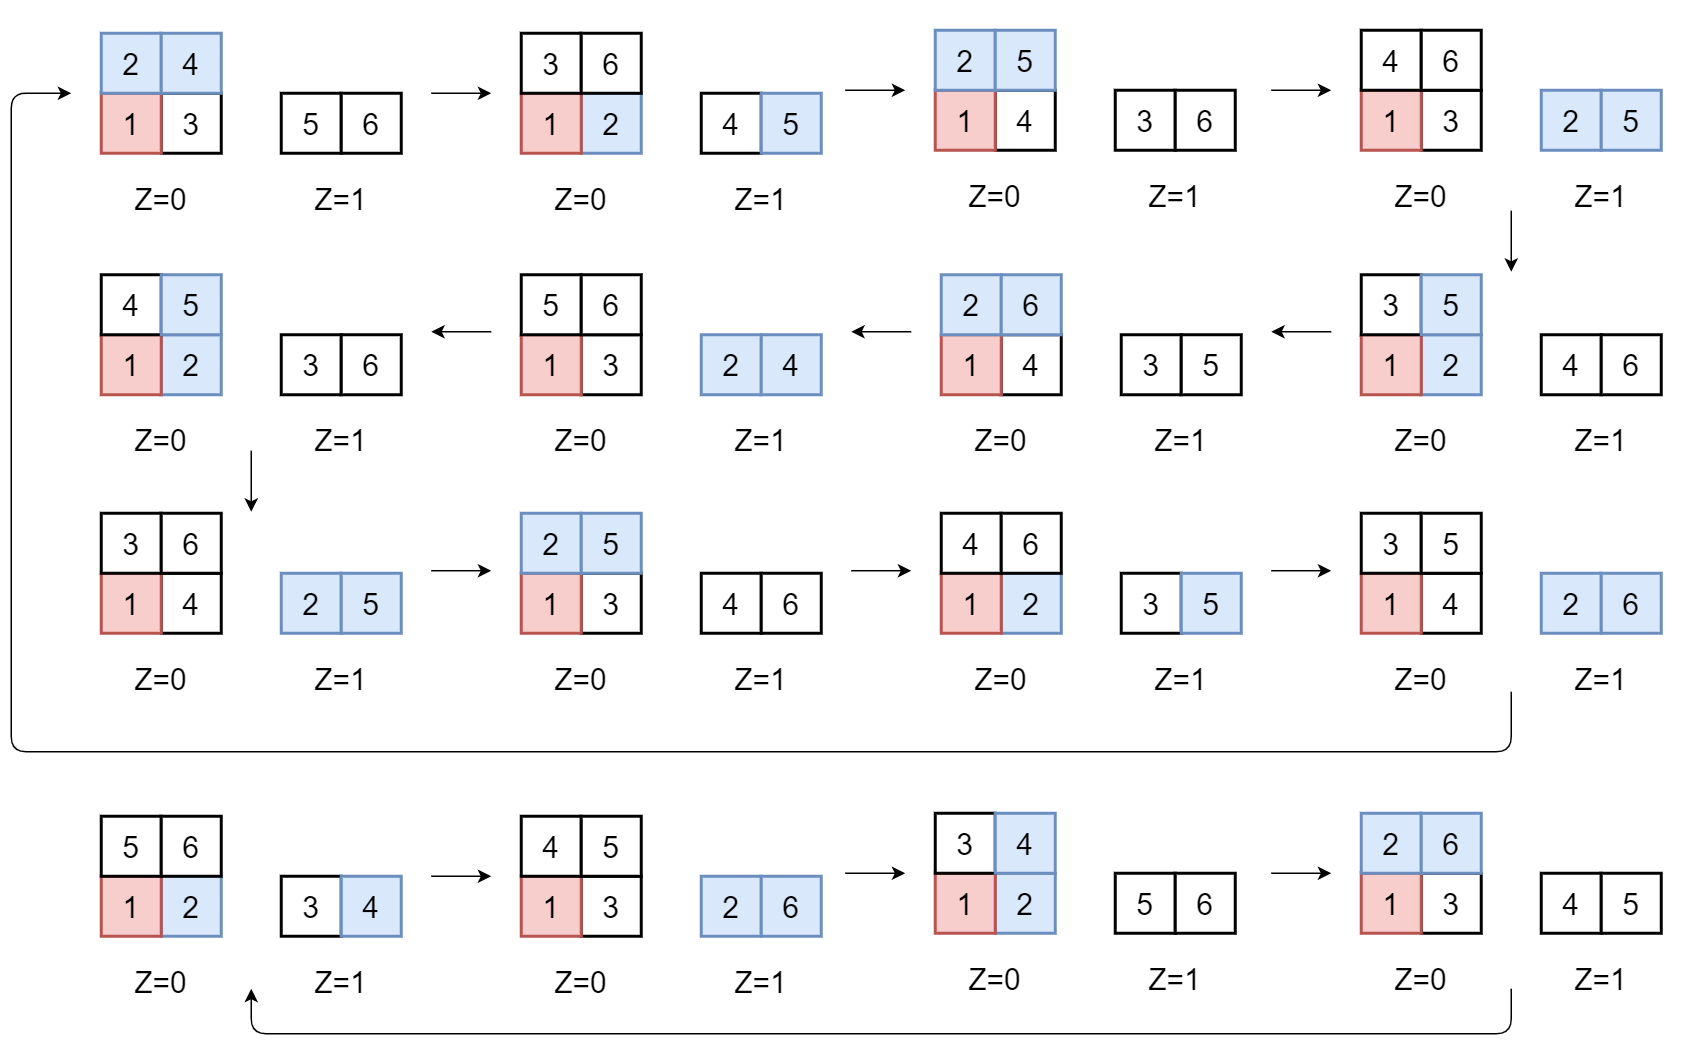
\includegraphics[scale=0.5]{./media/3.3.3_3.png}}
\end{figure}

\newpage

\section*{Теоретические сведения}

\subsection*{Задача 1.1}

Разбиение числа $n$ — это способ записать натуральное число $n$ в виде суммы натуральных чисел. При этом порядок слагаемых не учитывается, т.е. способы, отличающиеся только порядком слагаемых, считаются одним разбиением. Если порядок учитывается, то говорят о \textit{композициях} числа $n$. Для разбиений можно выбрать любой порядок слагаемых; канонической считается запись в виде невозрастающей последовательности положительных целых.

\noindent\textbf{Примеры:}

Например, $(3,1,1)$ или $(3,2)$ — разбиения числа 5, поскольку$ 5=3+1+1=3+2$. Всего есть 7 разбиений числа 5: $(1,1,1,1,1)$, $(2,1,1,1)$, $(2,2,1)$, $(3,1,1)$, $(3,2)$, $(4,1)$, $(5)$.

\subsubsection*{Получение теоремы Эйлера}

Производящая формула для числа разбиений $p(n)$ (формула Эйлера) имеет следующий вид:
\[ \sum_{n=0}^\infty p(n)x^n = \prod_{k=1}^\infty \left(\frac {1}{1-x^k} \right) \]

Рассмотрим следующее бесконечное произведение:
\[ (1 + x + x^2 + \dots)(1 + x^2 + x^4 + \dots)(1 + x^k + x^{2l} + \dots) \dots \]
После раскрытия скобок каждый член произведения получается в результате умножения мономов (одночленов), взятых по одному из каждой скобки. Если в первой скобке взять $x^{m_1}$, во второй - $x^{2m_2}$ и т.д., то их произведение будет равно $x^{m_1 + 2m_2 + 3m_3 + \dots}$. Значит, после раскрытия скобок получится сумма мономов данного вида.

Можно увидеть, что $x_n$ встретится в полученной бесконечной сумме столько раз, сколькими способами можно представить $n$ как сумму $m_1 + 2m_2 + 3m_3 + \dots$. Каждому такому представлению отвечает разбиение числа $n$ на $m_1$ единиц, $m_2$ двоек и т.д. Таким образом, очевидно, получаются все разбиения, так как из первой скобки мы можем взять любое $x^{m_i}$, где $m_i \in [0 \dots \infty]$, то есть произвольное количество единиц в нашем разбиении. Аналогично, мы можем взять произвольное количество двоек и т.д. Но при раскрытии скобок мы находим произведения всех возможных комбинации множителей из разных скобок. Поэтому коэффициент при $x^n$ равен числу разбиений $p(n)$.

Посмотрим теперь на выражения в скобках. Каждое из них — бесконечная геометрическая прогрессия. Полагая $0 \le x < 1$, по формуле ее суммирования:
\begin{align}
	& 1 + x + x^2 + x^3 + \dots = \dfrac{1}{1 - x} \\
	& 1 + x^2 + x^4 + x^6 + \dots = \dfrac{1}{1 - x^2} \\
	& \dots \\
	& 1 + x^k + x^{2k} + x^{3k} + \dots = \dfrac{1}{1 - x^k} \\
	& \dots \\
\end{align}

Запишем теперь производящую функцию последовательности $p(n)$:
\begin{equation}\label{formula:first}
p(0) + p(1)x + p(2)x^2 + p(3)x^3 + \dots = \dfrac{1}{(1-x)(1-x^2)(1-x^3) \dots}
\end{equation}

Рассмотрим произведение $(1 - x)(1 - x^2)(1 - x^3) \dots$, т.е. знаменатель правой части формулы \eqref{formula:first}. Раскрывая в нём скобки, получим следующий:
\[ (1 - x)(1 - x^2)(1 - x^3) \dots = 1 - x - x^2 + x^5 + x^7 - x^{12} - x^{15} + x^{22} + x^{26} - x^{35} - x^{40} + \dots \]

Показатели степеней в правой части — пятиугольные числа, т.е. числа вида $\dfrac{3q^2 \pm q}{2}$, а знаки при соответствующих мономах равны $(-1)^q$.

\begin{theorem}[Пентагональная теорема Эйлера]
	\[ \prod_{k=1}^{\infty} (1 - x^k) = \sum_{q = - \infty}^{\infty} (-1)^q x^{\frac{3q^2+q}{2}} \]
\end{theorem}

\begin{theorem}[Переформулировка пентагональной теоремы]
	Если число $N$ не может быть представлено в виде $N = \dfrac{3q^2+q}{2}$, то оно имеет одинаковое количество разбиений на четное и на нечетное число различных слагаемых. А для чисел вида $N = \dfrac{3q^2+q}{2}$ разность между этими количествами равна $(-1)^q$.
	
	Иными словами, если $q$ четно, то на одно больше разбиений на четное число слагаемых, а если $q$ нечетно, то на одно больше разбиений на нечетное число слагаемых.
\end{theorem}

Умножим обе части равенства \eqref{formula:first} на $\prod\lim\limits_{k=1}^{\infty}(1-x^k)$ и воспользуемся пентагональной теоремой:
\begin{equation}\label{formula:second}
(P(0) + p(1)x + p(2)x^2 + \dots)(1 - x - x^2 + x^5 + x^7 - x^{12} - x^{15} + \dots) = 1
\end{equation}
Начнем раскрывать скобки, для наглядности мономы с одинаковыми степенями $x$ пишем друг под другом:
\begin{align}
p(0) + &p(1)x + &p(2)x^2 + &p(3)x^3 + &p(4)x^4 + &p(5)x^5 + &p(6)x^6 + \dots \\
	   &-p(0)x - &p(1)x^2 + &p(2)x^3 - &p(3)x^4 + &p(4)x^5 + &p(5)x^6 + \dots \\
	   &	     & p(0)x^2 + &p(1)x^3 - &p(2)x^4 + &p(3)x^5 + &p(4)x^6 + \dots \\
	   &		 &	 		 &	        &		   &p(0)x^5 + &p(1)x^6 + \dots
\end{align}

Так как $p(0) = 1$, то оно сокращается с единицей справа. Так что, чтобы выражение \eqref{formula:second} было удовлетворено при любом $x$, все коэффициенты должны быть равны 0. Поэтому:
\[p(1) = p(0); p(2) = p(1) + p(0); p(3) = p(2) + p(1); p(4) = p(3) + p(2); p(5) = p(4) + p(3) - p(0)\]

\noindent\textbf{Формула Эйлера}, позволяющая последовательно находить числа $p(n)$:
\[ p(n) = p(n - 1) + p(n - 2) + \dots + (-1)^{q+1} \left( p \left(n - \dfrac{3q^2-q}{2}\right) + p \left(n - \dfrac{3q^2+q}{2}\right) \right) \]

Асимптотика: $O(n \sqrt{n})$. Т.к. $n - \dfrac{3q^2+q}{2} \ge 0$, то получаем $q$ порядка $\sqrt{n}$, а так как находим $n$-е число, то получаем приведённую оценку.

\end{document} 